\documentclass[parskip,12pt]{beamer}
% \documentclass[parskip,12pt, handout]{beamer}

\usetheme{Glasgow3}
%\usetheme[eco]{Glasgow3}
%\usepackage{handoutWithNotes}
%\pgfpagesuselayout{4 on 1 with notes}[a4paper,border shrink=5mm]

\usefonttheme[mathonly]{serif}
\usepackage{wasysym}
\usepackage[utf8]{inputenc}
\usepackage{pgf,pgfarrows,pgfnodes,pgfautomata,pgfheaps,pgfshade}
\usepackage{verbatim}
\usepackage{times}
\usepackage{dsfont,amsmath,amsfonts,xspace}
\usepackage[metapost]{mfpic}
\newcommand{\rr}{\ensuremath{\mathbb{R}}}
\newcommand{\nn}{\ensuremath{\mathbb{N}}}
\newcommand{\ee}{\ensuremath{\mathds{E}}}
\newcommand{\pp}{\ensuremath{\mathds{P}}}
\newcommand{\vv}{\ensuremath{\mathrm{Var}}}
\newcommand{\var}[2][]{\ensuremath{\vv_{#1}\left( #2 \right)}\xspace}
\newcommand{\oneone}{\ensuremath{\mathds{1}}}
\newcommand{\dist}[1]{\ensuremath{\mathsf{#1}}}
\usepackage{yfonts}
\usepackage{lettrine}
\usepackage{media9}
\usepackage{multimedia}
\graphicspath{{figures/}}
\newcommand{\compl}[1]{#1^{\complement}}
\usepackage{changepage}
\setbeamercolor{bgcolor}{fg=white,bg=uogblue}

\AtBeginSection[]{
  \begin{frame}
  \vfill
  \centering
  \begin{beamercolorbox}[sep=8pt,center,shadow=true,rounded=true]{bgcolor}
    \usebeamerfont{title}\insertsectionhead\par%
  \end{beamercolorbox}
  \vfill
  \end{frame}
}


\providecommand{\var}[1]{\operatorname{Var}\bigl(#1\bigr)}
\providecommand{\cov}[1]{\operatorname{Cov}\bigl(#1\bigr)}
\providecommand{\Var}[1]{\operatorname{Var}\left(#1\right)}
\providecommand{\Cov}[1]{\operatorname{Cov}\left(#1\right)}
\newcommand{\mub}{\mbox{{\boldmath $\mu$}}}
\newcommand{\sigmab}{\mbox{{\boldmath $\sigma$}}}
\newcommand{\Sigmab}{\mbox{{\boldmath $\Sigma$}}}
\newcommand{\betab}{\mbox{{\boldmath $\beta$}}}
\newcommand{\alphab}{\mbox{{\boldmath $\alpha$}}}
\newcommand{\thetab}{\mbox{{\boldmath $\theta$}}}
\newcommand{\bd}[1]{\ensuremath{\mbox{\boldmath $#1$}}}

\pdfinfo
{
  /Title       (Environmental Statistics Week 6)
  /Creator     (TeX)
  /Author      (Craig Anderson)
}

\title{Environmental Statistics}
\subtitle{Week 7: Introduction to Spatial Ecology}
\author{Jafet Belmont}
\date{}

\begin{document}


\begin{frame}
\frametitle{\textcolor{orange}{Late Night Talking}}
\center{

\includegraphics[scale=0.22]{Menti-W6-1}\\
}
\vspace{-3mm}
\url{https://www.menti.com/alz6g6hw4mr7}
\end{frame}

\begin{frame}
\frametitle{\textcolor{orange}{Meet Me in the Hallway}}
 \begin{itemize}
\item In the last two weeks, we looked at time series - data which vary over \emph{time}.
\vspace{3mm}
\item We noted that observations closer together in time were likely to be correlated, and we discussed methods for accounting for that correlation.
\vspace{3mm}
\item Over the next two weeks, we will look at data which vary over \emph{space}.
\vspace{3mm}
\item This takes us into the field of spatial statistics, which focuses on developing methods to account for spatial correlation. 
\end{itemize}
\end{frame}

\section{Introduction to Spatial Statistics}

\begin{frame}
\frametitle{\textcolor{orange}{Late Night Talking}}
\center{

\includegraphics[scale=0.22]{Menti-W6-1}\\
}
\vspace{-3mm}
\url{https://www.menti.com/alz6g6hw4mr7}
\end{frame}

\begin{frame}
\frametitle{\textcolor{orange}{Satellite}}
\begin{itemize}
\item Spatial data are data which have any form of geographical information attached to them.
\vspace{3mm}
\item Spatial data are becoming increasingly frequent as a result of new technology (eg satellite weather data, GPS enabled devices including phones, CCTV systems).
\vspace{3mm}
\item Most environmental variables of interest will vary over space to some degree, for example global temperature, air pollution, species distribution.
\vspace{3mm}
\item We will typically use this spatial information to help us understand the relationship between our data points
\end{itemize}
\end{frame}

\begin{frame}
\frametitle{Spatial data}
 \begin{itemize}
\item Generally, each datapoint will contain a measured value in addition to information about their location (typically represented by some form of coordinate system).
\vspace{3mm}
\item However, in some cases the locations themselves will be our data (eg the positions of trees in a forest).
\vspace{3mm}
\item We typically assume that we have some degree of spatial autocorrelation present in our data.
\vspace{3mm}
\item Tobler's first law of geography states that:\\ \textcolor{blue}{\emph{“Everything is related to everything else, but near things are more related than distant things”}}
\end{itemize}
\end{frame}


\begin{frame}
\frametitle{\textcolor{orange}{Sign of the Times}}
 \begin{itemize}
 \vspace{3mm}
\item Air pollution levels are measured at monitoring stations around Glasgow.
\vspace{3mm}
\item 1 is ``\emph{Low}'' and 10 is ``\emph{Very High}''.
\end{itemize}
\begin{columns}
\begin{column}{0.5\textwidth}
    \begin{center}
    \textbf{17th July 2022}
     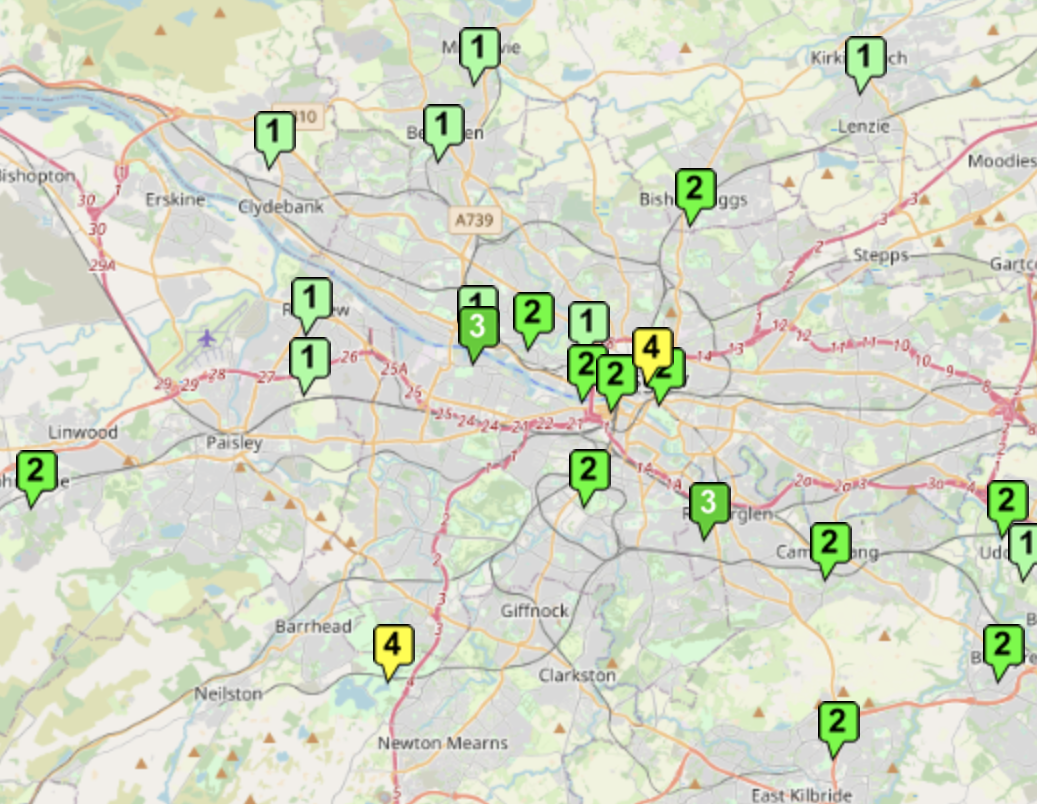
\includegraphics[width=\textwidth]{GlasgowMap}
          \end{center}
\end{column}
\begin{column}{0.5\textwidth}
    \begin{center}
    \textbf{17th January 2023}
     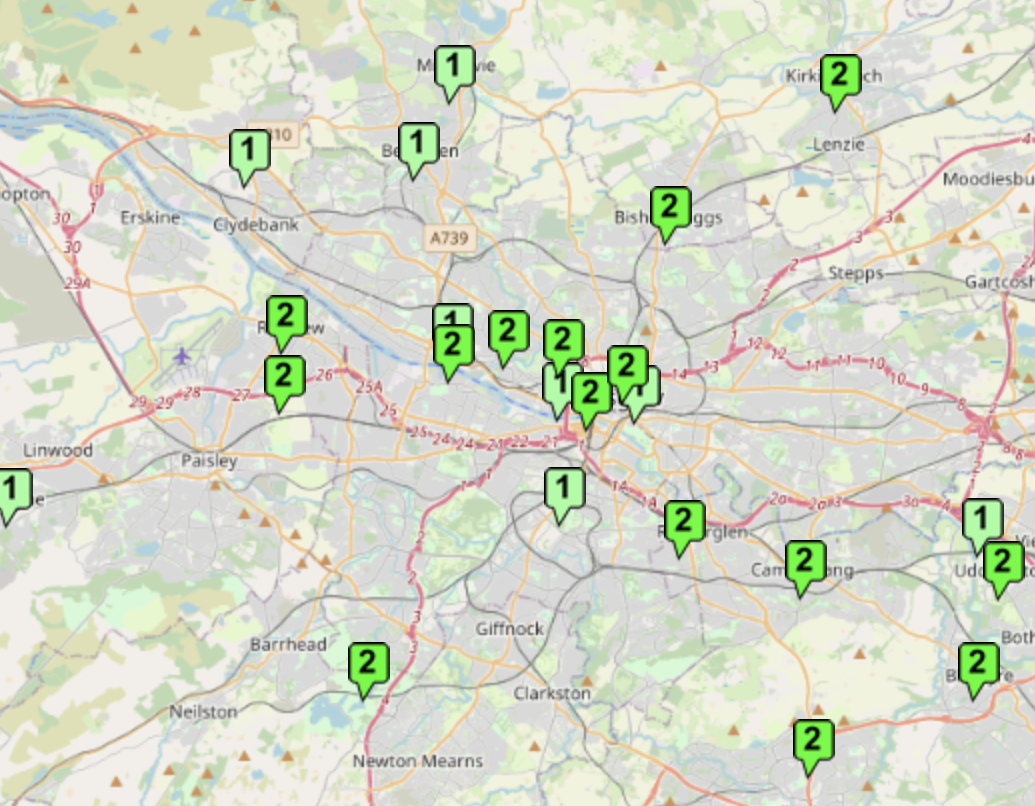
\includegraphics[width=\textwidth]{GlasgowMap2}
          \end{center}
\end{column}
\end{columns}
\vspace{2mm}
\url{https://www.scottishairquality.scot}
\end{frame}


\begin{frame}
\frametitle{Goals of spatial analysis}
 \begin{itemize}
\item The overall goal of any piece of spatial analysis is to understand the spatial patterns in our data.
\vspace{3mm}
\item This could involve any of the following:
\vspace{2mm}
\begin{itemize}
\item Estimating differences in mean, variance or some other summary statistic over space.
\vspace{2mm}
\item Predicting the value at some unobserved location.
\vspace{2mm}
\item Identifying ``hotspots'' with a high (or low) value compared to the rest of the region.
\end{itemize}
\vspace{3mm}
\item Typically this involves understanding and accounting for spatial autocorrelation in our data.
\end{itemize}
\end{frame}


\begin{frame}
\frametitle{Types of spatial data}
 \begin{itemize}
\item There are three main categories of spatial data which we will look at during this course.
\vspace{3mm}
\item These are geostatistical data, point processes and areal (or lattice) data.
\vspace{3mm}
\item We will briefly introduce each of them and identify the main topics where they are used for environmental data.
\vspace{3mm}
\item Note that there is a separate Spatial Statistics course which covers each of these types of data in more detail.
\end{itemize}
\end{frame}


\begin{frame}
\frametitle{Geostatistical data}
 \begin{itemize}
\vspace{3mm}
\item Measurements are taken at a set of fixed locations to measure some continuous process.
\end{itemize}
\begin{columns}
\begin{column}{0.5\textwidth}
    \begin{center}
    \textbf{Air pollution in Glasgow}
     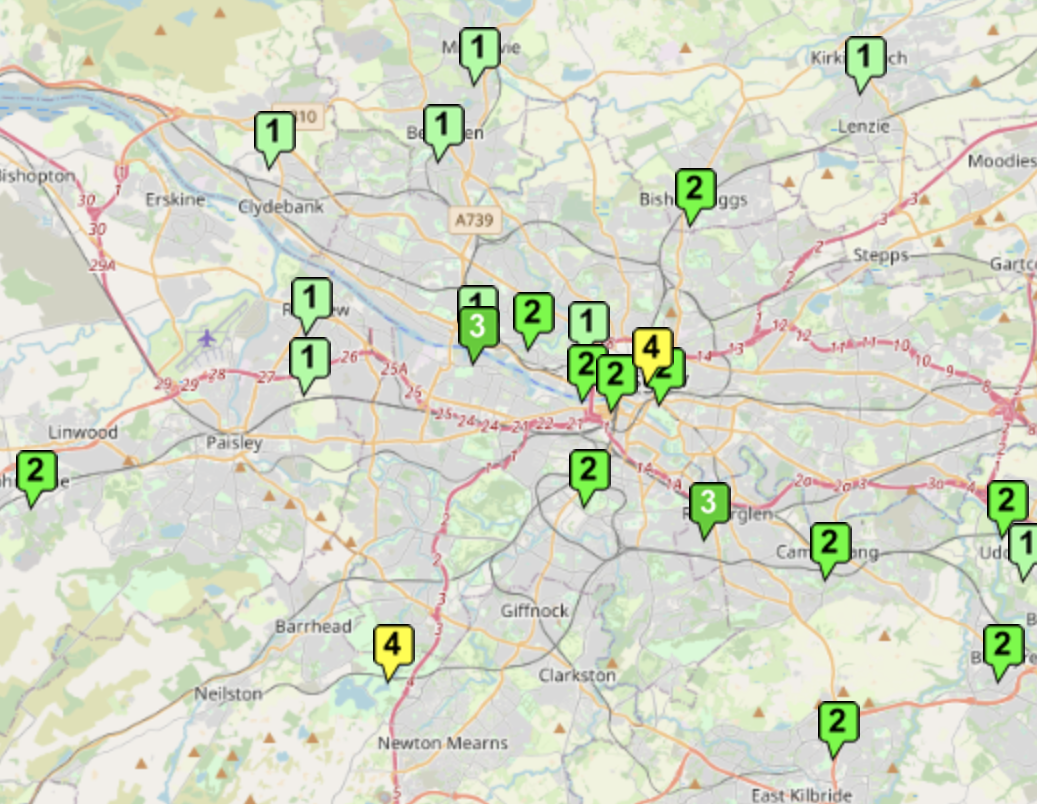
\includegraphics[width=\textwidth]{GlasgowMap}
          \end{center}
\end{column}
\begin{column}{0.5\textwidth}
    \begin{center}
    \textbf{Bathing water quality in Mallorca}
     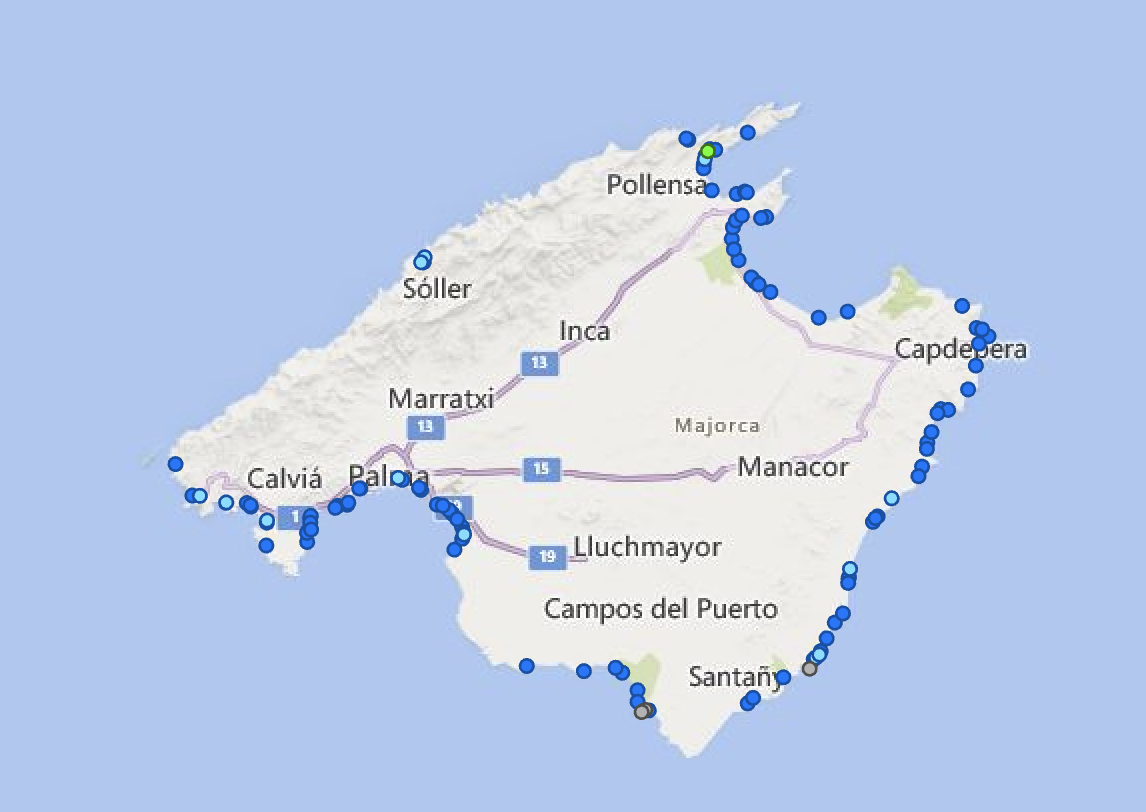
\includegraphics[width=\textwidth]{MallorcaBeaches}
          \end{center}
\end{column}
\end{columns}
\vspace{2mm}
\footnotesize{\url{https://www.eea.europa.eu/themes/water/interactive/bathing/state-of-bathing-waters}}
\end{frame}


\begin{frame}
\frametitle{Point process}
 \begin{itemize}
\vspace{3mm}
\item We measure the locations where events occur (eg trees in a forest, earthquakes) and the coordinates are our data.
\end{itemize}
\begin{columns}
\begin{column}{0.5\textwidth}
    \begin{center}
    \textbf{Locations of flowers}
     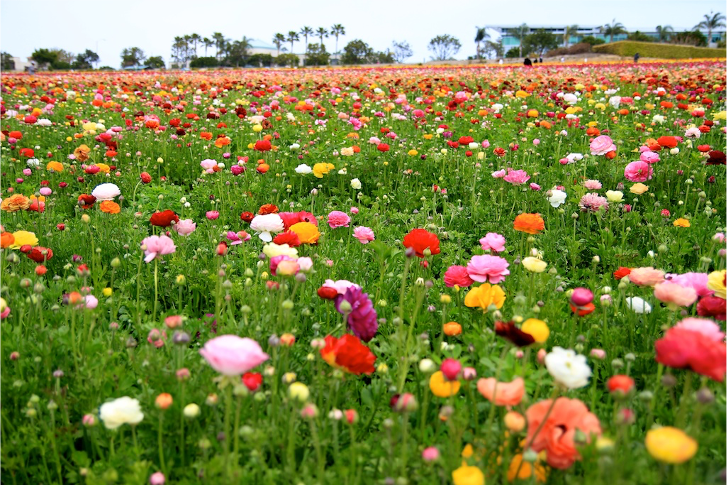
\includegraphics[width=\textwidth]{Flowers}
          \end{center}
\end{column}
\begin{column}{0.5\textwidth}
    \begin{center}
    \textbf{Forest fires in Castilla La Mancha, Spain}
     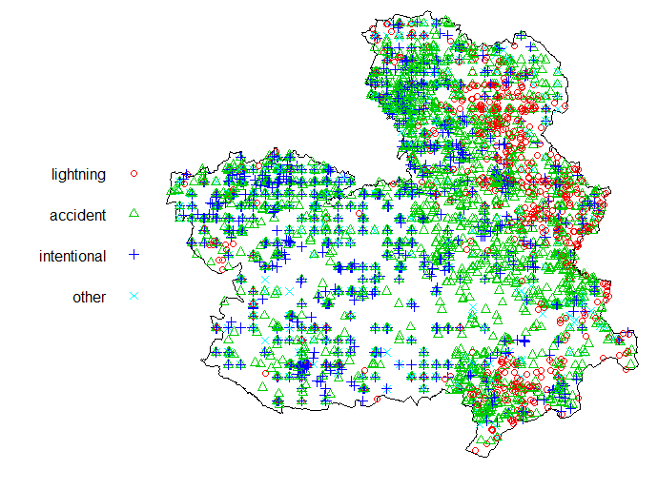
\includegraphics[width=\textwidth]{Fires}
          \end{center}
\end{column}
\end{columns}
\end{frame}


\begin{frame}
\frametitle{Areal}
 \begin{itemize}
\vspace{3mm}
\item Our data are measured as a summaries across a set of discrete, non-overlapping spatial units (eg postcode areas, council regions).
\end{itemize}
\begin{columns}
\begin{column}{0.5\textwidth}
    \begin{center}
    \textbf{Pollution in English local authorities}
     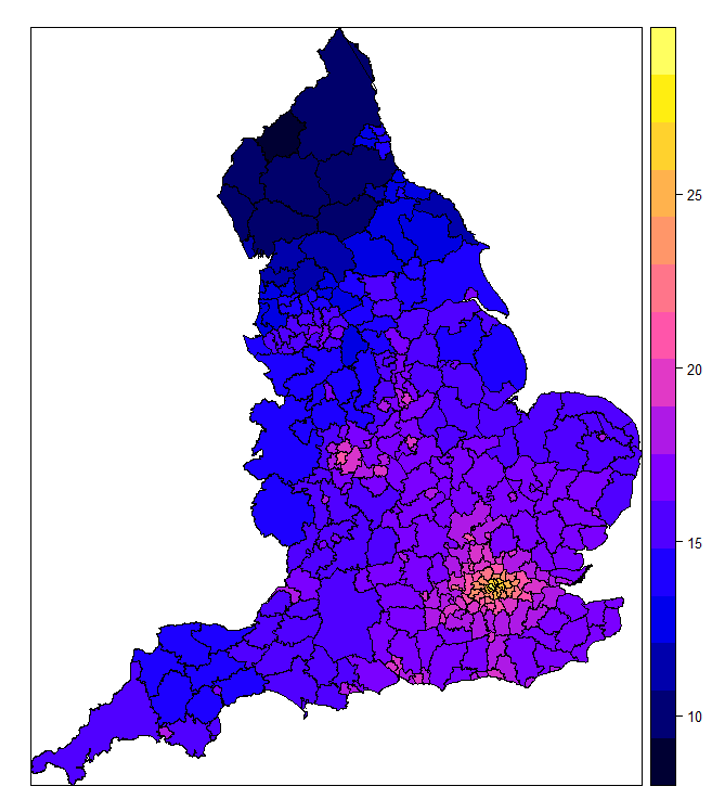
\includegraphics[width=0.7\textwidth]{EnglandPollution}
          \end{center}
\end{column}
\begin{column}{0.5\textwidth}
    \begin{center}
    \textbf{Human respiratory disease in Glasgow}
     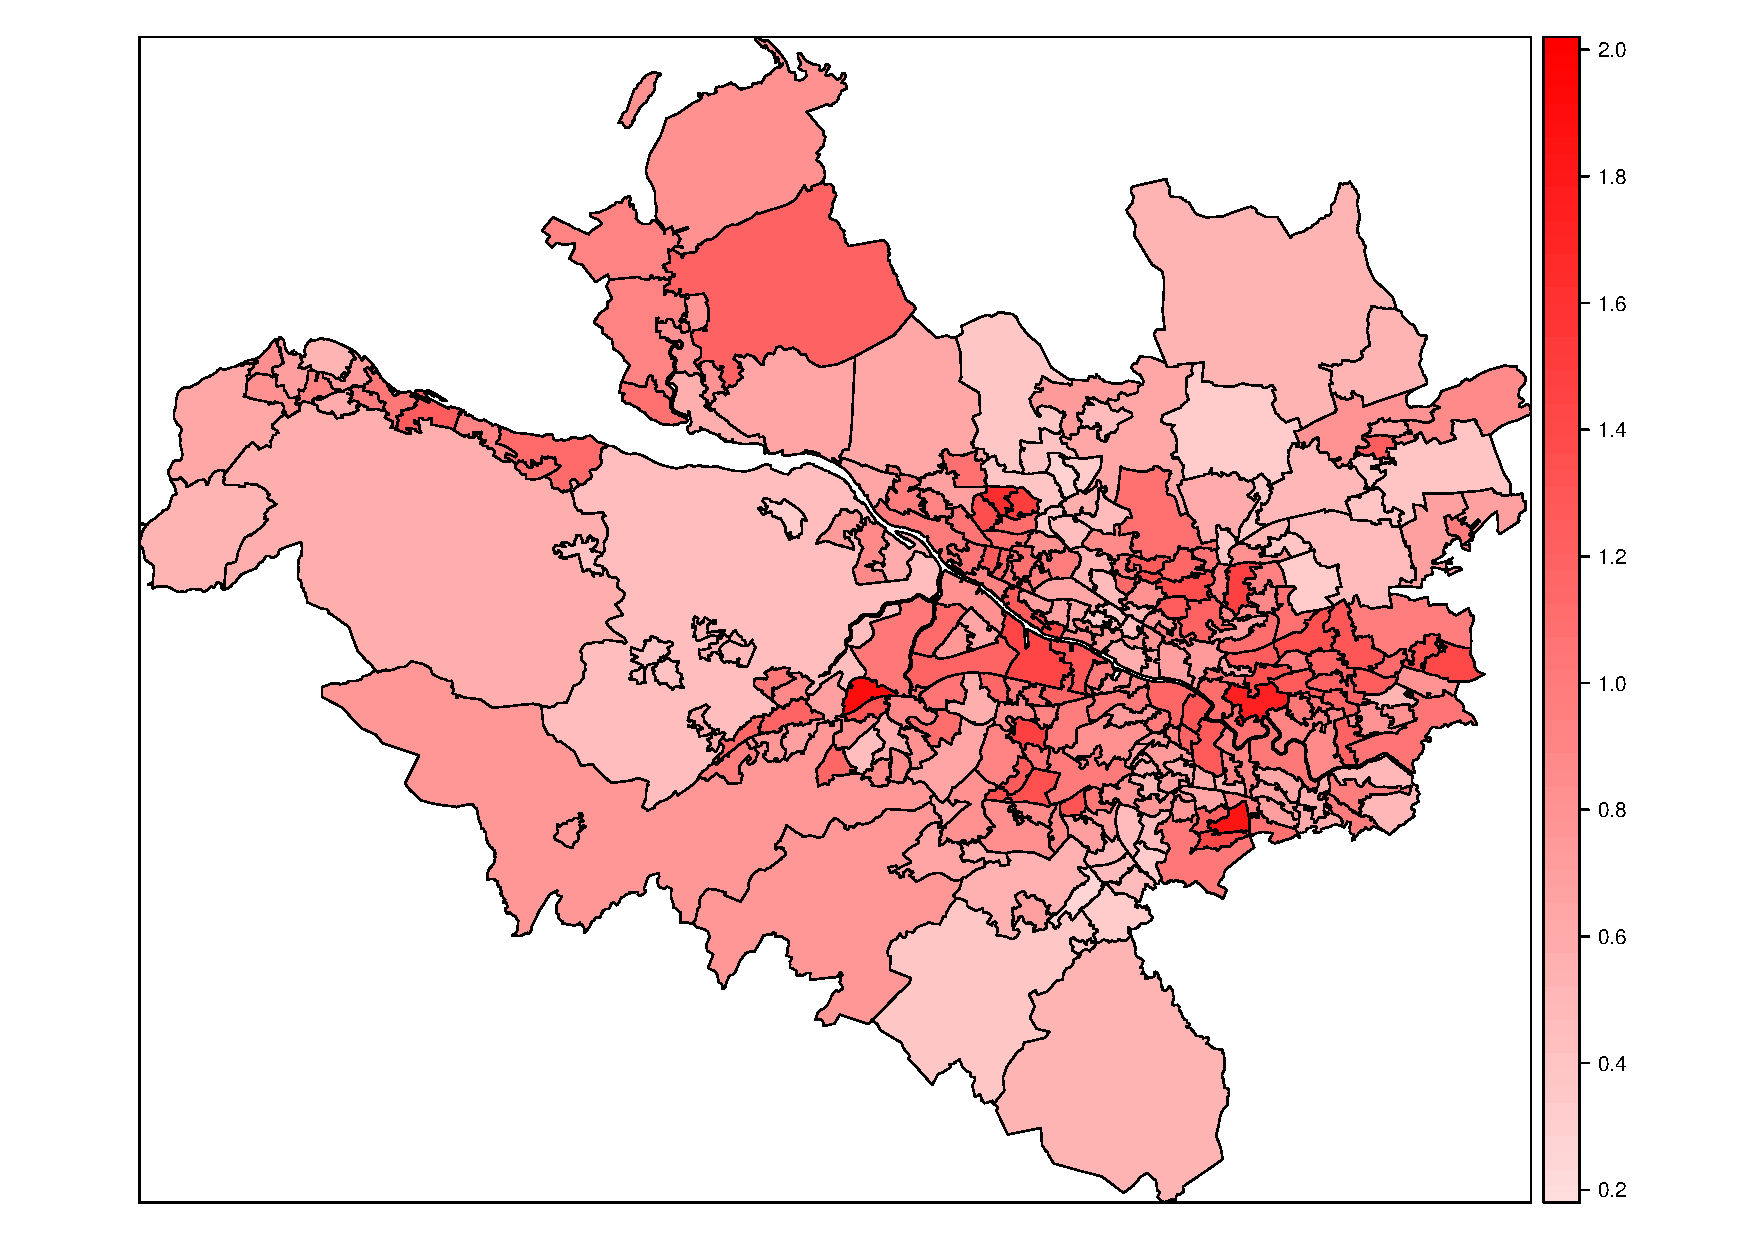
\includegraphics[width=\textwidth]{GlasgowResp}
          \end{center}
\end{column}
\end{columns}
\end{frame}


\section{Introduction to Geostatistical Data}

\begin{frame}
\frametitle{Geostatistical data}
 \begin{itemize}
\item Geostatistical data are the most common form of spatial data found in environmental setting.
\vspace{3mm}
\item We regularly take measurements of an environmental variable of interest at a set of fixed locations.
\vspace{3mm}
\item This could be data from samples taken across a region (eg water depth in a lake) or from monitoring stations as part of a network (eg air pollution).
\vspace{3mm}
\item In each of these cases, our goal is to estimate the value of our variable across the entire space.
\end{itemize}
\end{frame}


\begin{frame}
\frametitle{Understanding our region}
 \begin{itemize}
\item Let $D$ be our two-dimensional region of interest.
\vspace{3mm}
\item In principle, there are infinite locations within $D$, each of which can be represented by mathematical coordinates (eg latitude and longitude).
\vspace{3mm}
\item We can identify any individual location as $\bd{s}_i = (x_i, y_i)$, where $x_i$ and $y_i$ are their coordinates.
\vspace{3mm}
\item We can treat our variable of interest as a random variable, $Z$ which can be observed at any location as $Z(\bd{s}_i)$.
\end{itemize}
\end{frame}


\begin{frame}
\frametitle{Geostatistical process}
 \begin{itemize}
\item Our geostatistical process can therefore be written as: $$\{Z(\bd{s}); \bd{s} \in D\}$$
\item In practice, our data are observed at a finite number of locations, $m$, and can be denoted as: $$z = \{z(\bd{s}_1), \ldots z(\bd{s}_m) \}$$
\item We have observed our data at $m$ locations, but often want to predict this process at a set of unknown locations.
\vspace{3mm}
\item For example, what is the value of $z(\bd{s}_0)$, where $\bd{s}_0$ is an unobserved site?
\end{itemize}
\end{frame}

\begin{frame}
\frametitle{Geostatistical analysis}
 \begin{itemize}
\item There are two main steps in classical geostatistical analysis.
\vspace{2mm}
\begin{enumerate}
\item How do I produce a statistical model for the data?
\vspace{2mm}
\item How do I use my model to estimate quantities of interest?
\end{enumerate}
\vspace{3mm}
\item The first part requires us to think about how our measured datapoints relate to each other - in other words, to understand spatial autocorrelation.
\vspace{3mm}
\item The second part requires us to use that information to predict the value at unmeasured locations, and then to produce maps or summary statistics based on this.
\end{itemize}
\end{frame}


\begin{frame}
\frametitle{Example: River nitrogen}
 \begin{itemize}
\vspace{3mm}
\item We are interested in nitrate levels in the River Trent.
\vspace{3mm}
\item A set of locations in the river network are sampled.
\end{itemize}
\begin{columns}
\begin{column}{0.56\textwidth}
\begin{itemize}
\item There are UK/EU directives for safe nitrate levels in water bodies such as rivers.
\vspace{3mm}
\item Our goal is to answer a \textbf{policy} question - which areas breach 50mg/l limit?
\vspace{3mm}
\item This requires us to estimate the levels at unmeasured locations.
\end{itemize}
\end{column}
\begin{column}{0.32\textwidth}
    \begin{center}
     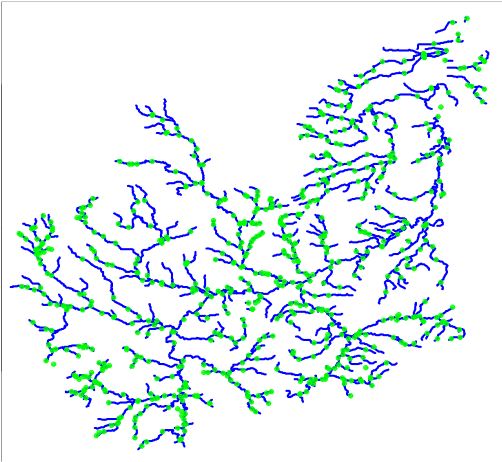
\includegraphics[width=\textwidth]{TrentNetwork}\\
     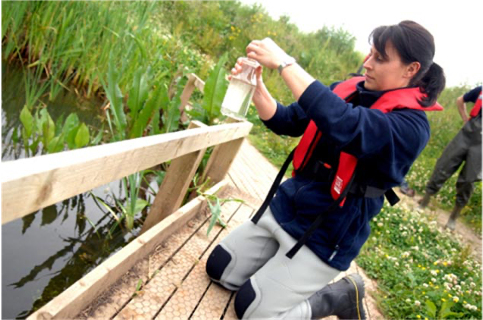
\includegraphics[width=\textwidth]{WaterSampling}
          \end{center}
\end{column}
\end{columns}
\end{frame}


\begin{frame}
\frametitle{Example: River nitrogen}
 \begin{itemize}
\vspace{3mm}
\item The plot below shows the average nitrate levels from 2003-2010 at each of our observed locations.
\vspace{3mm}
\item Darker colours and larger plotting points correspond to higher levels of nitrate.
\end{itemize}
    \begin{center}
     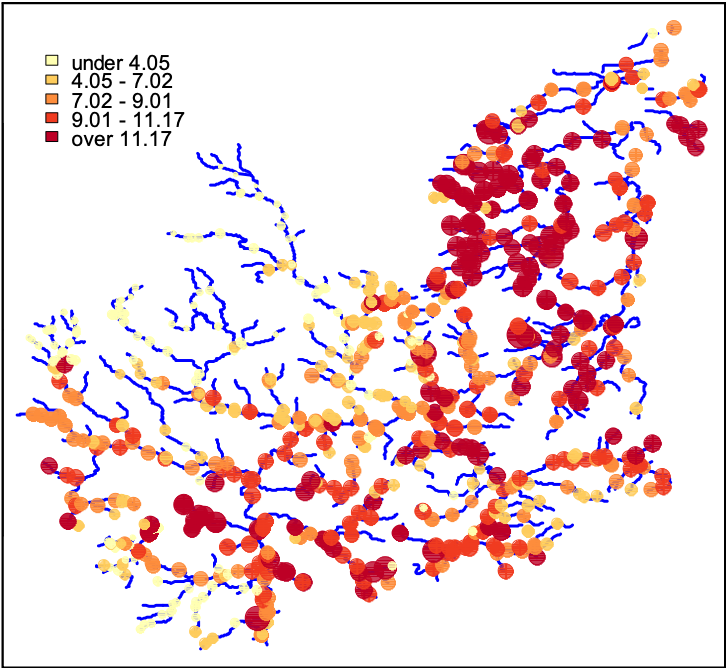
\includegraphics[width=0.5\textwidth]{TrentData}
          \end{center}
\end{frame}


\begin{frame}
\frametitle{\textcolor{orange}{Golden}}
\center{

\includegraphics[scale=0.22]{Menti-W6-1}\\
}
\vspace{-3mm}
\url{https://www.menti.com/alz6g6hw4mr7}
\end{frame}

\begin{frame}
\frametitle{\textcolor{orange}{To Be So Lonely}}
 \begin{itemize}
\vspace{3mm}
\item Visually, it appears that the highest levels are located in the north-east and far south of the region.
\vspace{3mm}
\item However, we require a statistical model to measure this objectively.
\end{itemize}
    \begin{center}
     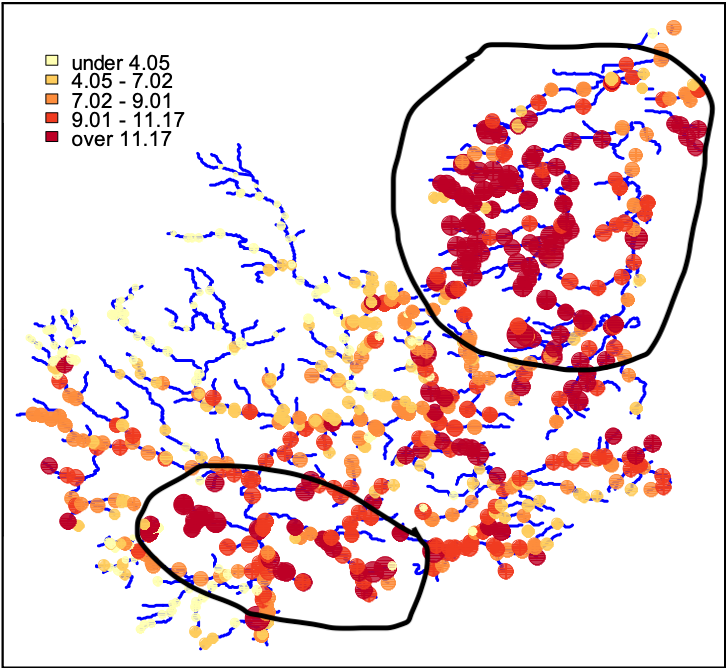
\includegraphics[width=0.5\textwidth]{TrentData2}
          \end{center}
\end{frame}


\begin{frame}
\frametitle{Modelling geostatistical data}
 \begin{itemize}
\item The key challenge in modelling geostatistical data is understanding \textbf{correlation}.
\vspace{3mm}
\item Typically observations close together in space will be more similar than those which are further apart.
\vspace{3mm}
\item Spatial correlation is usually driven by some unmeasured confounding variable(s) - for example, air pollution is spatially correlated because nearby areas tend to experience similar traffic levels.
\vspace{3mm}
\item It is important that we account for these correlations in our analysis - failing to do so will lead to poor inference.
\end{itemize}
\end{frame}

\begin{frame}
\frametitle{Modelling geostatistical data}
 \begin{itemize}
\item For a set of geostatistical data $\bd{z} = \{ z(\bd{s}_1), \ldots, z(\bd{s}_m) \}$, we can consider the general model: $$Z(\bd{s}_i) = \mu(\bd{s}_i) + e(\bd{s}_i)$$
\item Here $\mu(\bd{s}_i)$ is a mean function which models trend and covariate effects.
\vspace{3mm}
\item Then $e(\bd{s}_i)$ is the error process which accounts for any spatial correlation which exists after accounting for $\mu(\bd{s}_i)$
\vspace{3mm}
\item Spatial statistics is therefore often focused on understanding the process for $e(\bd{s}_i)$.
\end{itemize}
\end{frame}

\begin{frame}
\frametitle{Our key problem(s)}
 \begin{itemize}
\item We have observations at $m$ locations $$\bd{z} = \{ z(\bd{s}_1), \ldots, z(\bd{s}_m) \}.$$
\item We want to use these to obtain an estimate of $Z(\bd{s}_0)$ where $\bd{s}_0$ is an unobserved location.
\vspace{3mm}
\item How do we model the spatial dependence between our observed sites $\bd{s}_1, \ldots, \bd{s}_m$?
\vspace{3mm}
\item What does this tell us about the dependence between our observed sites and our unobserved site $\bd{s}_0$?
\end{itemize}
\end{frame}


\section{Variograms}

\begin{frame}
\frametitle{Modelling spatial dependence}
 \begin{itemize}
\item Spatial dependence is commonly modelled by a function known as a \textbf{variogram}.
\vspace{3mm}
\item The variogram is similar in many ways to the autocorrelation function used in time series modelling.
\vspace{3mm}
\item In simple terms, it is a function which measures the difference in the spatial process between a pair of locations a fixed distance apart.
\vspace{3mm}
\item In order to define the variogram, it is important to first understand some more features of a geostatistical process.
\end{itemize}
\end{frame}


\begin{frame}
\frametitle{Mean}
 \begin{itemize}
\item If we have a geostatistical process $\{Z(\bd{s}); \bd{s} \in D\}$, then its mean can be expressed as $$\mu_z(\bd{s}) = E[{Z(\bd{s})}] \mbox{ for all } \bd{s} \in D.$$
\item Our process $Z$ is then said to be Gaussian if our random variable at the set of observed locations is multivariate normal.
\vspace{3mm}
\item In other words, $Z$ is Gaussian if $$\{ Z(\bd{s_1}, \ldots, Z(\bd{s_m} \} \sim \mbox{MVN}(\mu_z(\bd{s}), C_z(\bd{s})).$$
\end{itemize}
\end{frame}


\begin{frame}
\frametitle{Variance and covariance}
 \begin{itemize}
\item Similarly, the covariance can be expressed as:
\begin{align*}
C_z(\bd{s}, \bd{t}) =& \Cov{Z(\bd{s}), Z(\bd{t})}\\
=& E\left[(Z(\bd{s}) - \mu_z(\bd{s}))(Z(\bd{t}) - \mu_z(\bd{t}))\right]
\end{align*}
\item Here, the covariance measures the strength of the linear dependence between $Z(\bd{s})$ and $Z(\bd{t})$.
\vspace{3mm}
\item As usual, we can compute the variance of $Z(\bd{s})$ as a special case of the covariance where $\bd{s} = \bd{t}.$
\end{itemize}
\end{frame}


\begin{frame}
\frametitle{Weak stationarity}
 \begin{itemize}
\item Our geostatistical process can be described as \textbf{weakly stationary} if the following criteria are met:
\vspace{2mm}
\begin{enumerate}
\item $E[{Z(\bd{s})}] = \mu_z(\bd{s}) = \mu_z$ - a finite constant which does not depend on $\bd{s}$.
\vspace{2mm}
\item $C_z(\bd{s}, \bd{s+h}) = C_z(\bd{h})$ - a finite constant which can depend on $\bd{h}$ but not $\bd{s}$.
\end{enumerate}
\vspace{2mm}
\item Condition 1 states that our mean function must be constant in space, with no overall spatial trend.
\vspace{3mm}
\item Condition 2 states that for any two locations, their covariance depends only on how far apart they are (their \textbf{spatial lag}, $h$), not their absolute position.
\end{itemize}
\end{frame}


\begin{frame}
\frametitle{Isotropy}
 \begin{itemize}
\item A geostatistical process is said to be \textbf{isotropic} if the covariance function is \emph{directionally invariant}.
\vspace{3mm}
\item This means that the covariance between two points a distance $h$ apart is the same no matter which direction you travel in.
\vspace{3mm}
\item Mathematically, this can be denoted by $$C_z(\bd{h}) = C_z(||\bd{h}||).$$
\end{itemize}
\end{frame}

\begin{frame}
\frametitle{\textcolor{orange}{Daylight}}
\center{

\includegraphics[scale=0.22]{Menti-W6-2}\\
}
\vspace{-3mm}
\url{https://www.menti.com/alws53ba6bzm}
\end{frame}

\begin{frame}
\frametitle{Limitations of this course}
 \begin{itemize}
\item In this course, we will only look at Gaussian, weakly stationary and isotropic processes.
\vspace{3mm}
\item This means that:
\vspace{2mm}
\begin{itemize}
\item This means our random variables across our observed locations follow a multivariate Gaussian distribution.
\vspace{2mm}
\item The mean of this distribution is constant over space.
\vspace{2mm}
\item The covariance of this distribution is only a function of the lag, not the position or direction of the points.
\end{itemize}
\vspace{2mm}
\item Other models do exist for more complex processes, but we will not explore these.
\end{itemize}
\end{frame}
  

\begin{frame}
\frametitle{Autocovariance}
 \begin{itemize}
\item The function describing the dependence between values of our process $Z$ separated by different lags is known as the \textbf{autocovariance function}.
\vspace{3mm}
\item This is similar to the autocorrelation function (ACF) used for temporal data.
\vspace{3mm}
\item In geostatistical models, a variant of this known as a \textbf{variogram} is typically used to estimate spatial relationships.
\end{itemize}
\end{frame}


\begin{frame}
\frametitle{Variogram}
 \begin{itemize}
\item The variogram measures the variance of the difference in the process at two spatial locations $\bd{s}$ and $\bd{s+h}.$
\vspace{3mm}
\item The variogram is defined as $$\mbox{Var}[Z(\bd{s}) - Z(\bd{s} + \bd{h})] = E[(Z(\bd{s}) - Z(\bd{s} + \bd{h}))^2] = 2\gamma_z(\bd{h}).$$
\vspace{-2mm}
\item Here, $2\gamma_z(\bd{h})$ is the variogram, but in practice we use the \textbf{semi-variogram}, $\gamma_z(\bd{h})$.
\vspace{3mm}
\item We use the semi-variogram because our points come in pairs, and the semi-variance is equivalent to the variance per point at a given lag.
\end{itemize}
\end{frame}

\begin{frame}
\frametitle{Notes on (semi)-variogram}
 \begin{itemize}
\item When the variance of the difference $Z(\bd{s}) - Z(\bd{t})$ is relatively small, then $Z(\bd{s})$ and $Z(\bd{t})$ are similar (spatially correlated).
\vspace{3mm}
\item When the variance of the difference $Z(\bd{s}) - Z(\bd{t})$ is relatively large, then $Z(\bd{s})$ and $Z(\bd{t})$ are less similar (closer to independence).
\vspace{3mm}
\item If our process is \emph{weakly stationary} and \emph{isotropic} we can show that $$\gamma_z(\bd{h}) = \sigma^2_z - C_z(\bd{h}).$$
\vspace{-1mm}
\item Therefore, if we know the covariance function, we can calculate the (semi)-variogram.
\end{itemize}
\end{frame}
  
\begin{frame}
\frametitle{What does the variogram look like?}
 \begin{itemize}
\item The plot below shows a typical variogram, with the variance increasing as the lag increases.
\end{itemize}
\begin{columns}
\begin{column}{0.45\textwidth}
  \begin{itemize}
\item The \textbf{sill} is the maximum variance as $h \to \infty$.
\vspace{1mm}
\item The \textbf{nugget} is the minimum variance as $h \to 0$.
\vspace{1mm}
\item The \textbf{range} is the distance to the sill.
\end{itemize}
\end{column}
\begin{column}{0.45\textwidth}
    \begin{center}
     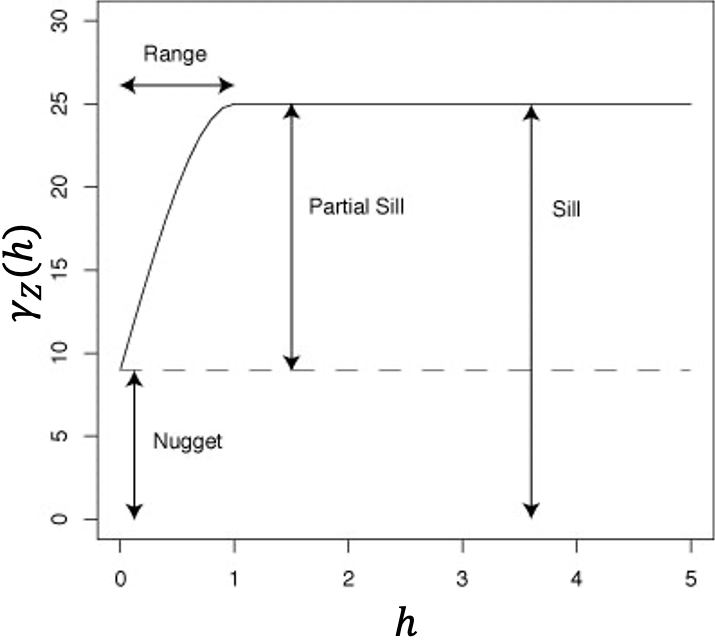
\includegraphics[width=\textwidth]{Variogram}
          \end{center}
\end{column}
\end{columns}
\vspace{3mm}
 \begin{itemize}
\item Points further apart than the range are assumed to be uncorrelated.
\end{itemize}
\end{frame}


\begin{frame}
\frametitle{Estimating the variogram}
 \begin{itemize}
\item The variogram is a function of the underlying geostatistical process $Z$.
\vspace{3mm}
\item In practice, we only have access to $m$ realisations of this process, and therefore we have to estimate the variogram.
\vspace{3mm}
\item This is known as the \emph{empirical variogram}.
\vspace{3mm}
\item We obtain this by computing the semi-variance for all possible pairs of observations: $\gamma(\bd{s}, \bd{t}) = 0.5(Z(\bd{s}) - Z(\bd{t}))^2$.
\vspace{3mm}
\item We can then plot the empirical variogram by plotting these semi-variances against their corresponding lags.
\end{itemize}
\end{frame}


\begin{frame}
\frametitle{Example - River Meuse}
 \begin{itemize}
\item We are interested in soil zinc levels in the flood plains of the River Meuse (in France, Belgium and the Netherlands).\\
\vspace{3mm}
\item Our goal is to model the spatial correlation in the data so that we can predict zinc levels at unsampled locations.
\end{itemize}
\vspace{-5mm}
\begin{columns}
\begin{column}{0.45\textwidth}
  \begin{itemize}
\item A set of sampling locations were selected.
\vspace{2mm}
\item Our data consist of location coordinates and zinc levels.
\end{itemize}
\end{column}
\begin{column}{0.45\textwidth}
    \begin{center}
     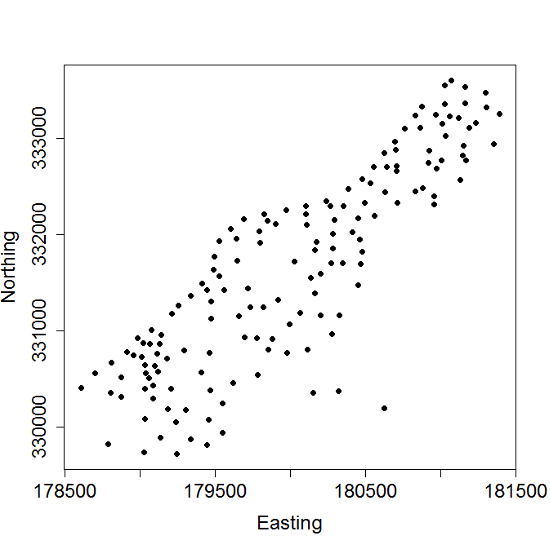
\includegraphics[width=\textwidth]{MeuseSamples}
          \end{center}
\end{column}
\end{columns}
\end{frame}

\begin{frame}
\frametitle{Example - River Meuse}
\vspace{1mm}    
    \begin{center}
     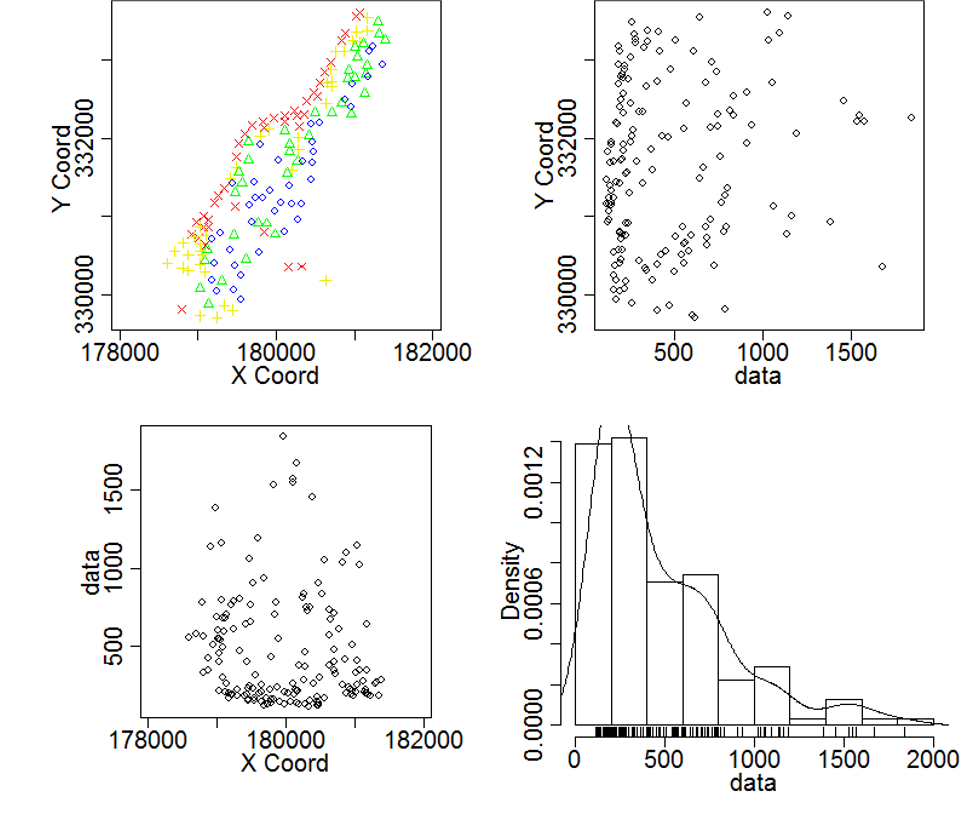
\includegraphics[width=0.7\textwidth]{MeuseRaw}
          \end{center}
\vspace{-2mm}          
Plots: (a) map colour coded by zinc level, (b) and (c) the zinc levels plotted against the x and y coordinates and (d) a density plot of the zinc levels.
\end{frame}

\begin{frame}
\frametitle{\textcolor{orange}{As It Was}}
\center{

\includegraphics[scale=0.22]{Menti-W6-2}\\
}
\vspace{-3mm}
\url{https://www.menti.com/alws53ba6bzm}
\end{frame}

\begin{frame}
\frametitle{\textcolor{orange}{Transforming our data}}
\vspace{1mm}    
    \begin{center}
     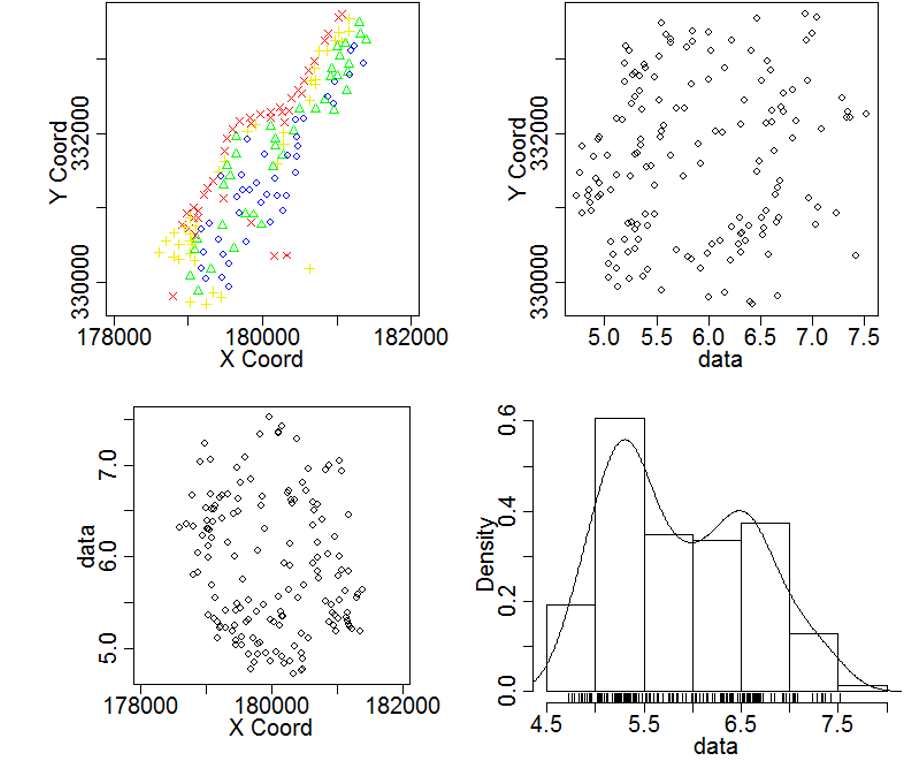
\includegraphics[width=0.7\textwidth]{MeuseLog}
          \end{center}
\vspace{-2mm}          
Plots: (a) map colour coded by \emph{log} zinc level, (b) and (c) the \emph{log} zinc levels plotted against the x and y coordinates and (d) a density plot of the \emph{log} zinc levels.
\end{frame}


\begin{frame}
\frametitle{Computing the empirical variogram}
\vspace{2mm}
 \begin{itemize}
\item To illustrate how an empirical variogram is computed, consider the two highlighted locations below.
\end{itemize}
    \begin{center}
     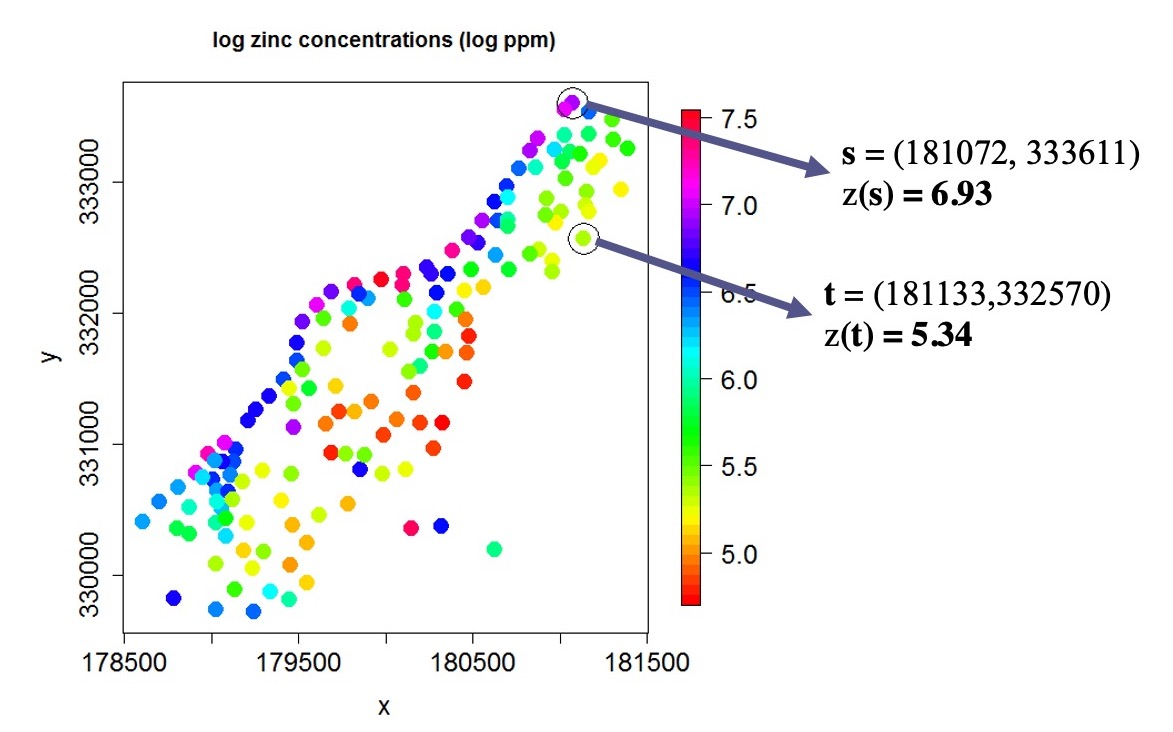
\includegraphics[width=\textwidth]{MeuseExample}
          \end{center}
\end{frame}

\begin{frame}
\frametitle{Computing the empirical variogram}
 \begin{itemize}
\item We can first compute the distance between the two locations using the standard Euclidean distance formula as \small{$$h = \sqrt{(181072-181133)^2 + (333611-332570)^2} = 1042.8$$}
\vspace{-2mm}
\item Next, we compute the semi-variance between the points using their observed values as
\begin{align*}
\gamma(\bd{s}, \bd{t}) =& 0.5(Z(\bd{s}) - Z(\bd{t}))^2\\
=& 0.5(6.93 - 5.34) = 1.27
\end{align*}
\vspace{-2mm}
\item We repeat this process for every possible pair of points, and plot $h$ against $\gamma(\bd{s}, \bd{t})$ for each.
\end{itemize}
\end{frame}

\begin{frame}
\frametitle{\textcolor{orange}{Daydreaming}}
\vspace{2mm}
 \begin{itemize}
\item This plot shows the semi-variances for each pair of points.
\vspace{2mm}
\item Each pair of points has a different distance, making it difficult to use this for prediction.
\vspace{-2mm}
\end{itemize}
    \begin{center}
     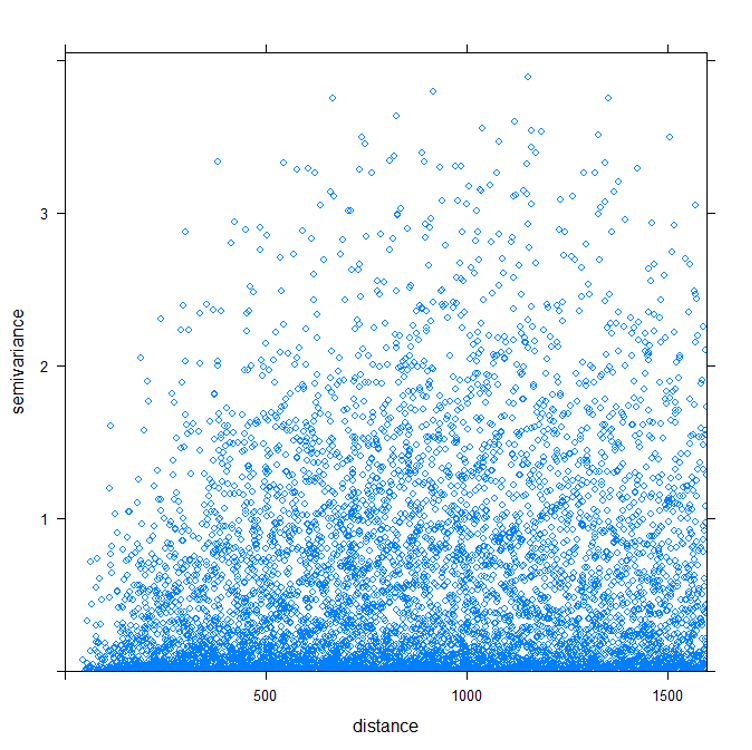
\includegraphics[width=0.6\textwidth]{MeuseVariogram}
          \end{center}
\end{frame}

\begin{frame}
\frametitle{Computing the empirical variogram}
 \begin{itemize}
\item To make the variogram easier to use and interpret, we divide the distances into a set of discrete bins, and compute the average semi-variance in each.
\vspace{3mm}
\item We compute this binned empirical variogram as $$\gamma(\bd{h}) = \frac{1}{2N(h_k)}\sum_{(\bd{s},\bd{t}) \in N(h_k)}[z(\bd{s}) - z(\bd{t})]^2$$
\item Here, $k$ is the number of bins and $N(h_k)$ is the number of points in the bin with average distance $h$.
\vspace{3mm}
\item We then construct a plot of our empirical variogram and use this to estimate the covariance structure.
\end{itemize}
\end{frame}


\begin{frame}
\frametitle{\textcolor{orange}{Fine Line}}
 \begin{itemize}
\item The bins are illustrated on the left, and the empirical variogram obtained from them is shown on the right.
\vspace{3mm}
\item We can start to think about estimating a nugget, sill and range based on this empirical variograrm.
\end{itemize}
\begin{columns}
\begin{column}{0.47\textwidth}
    \begin{center}
     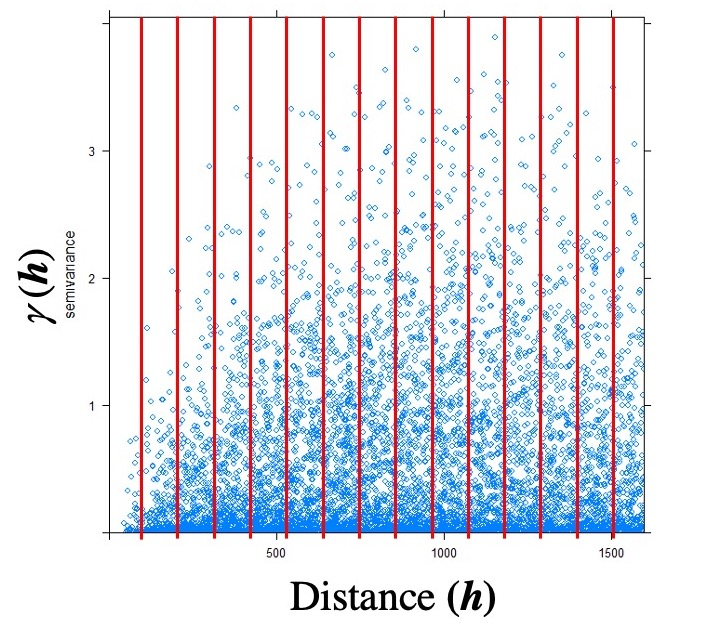
\includegraphics[width=\textwidth]{MeuseBinned}
          \end{center}
\end{column}
\begin{column}{0.53\textwidth}
    \begin{center}
     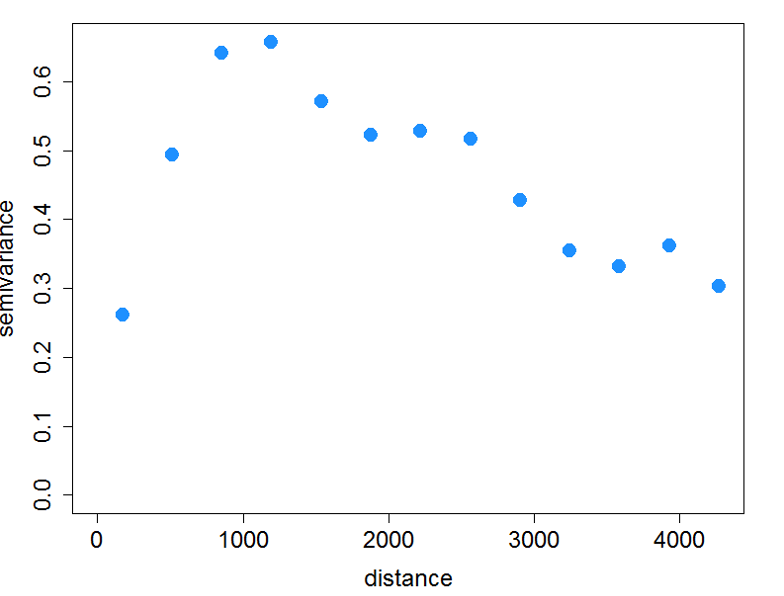
\includegraphics[width=\textwidth]{MeuseEmpirical}
          \end{center}
\end{column}
\end{columns}
\end{frame}


\begin{frame}
\frametitle{Fitting our model}
 \begin{itemize}
\item Once we have computed an empirical variogram, we have to think about fitting a model to it.\vspace{3mm}
\item We only have estimates at a small number of lags, we would like a continuous model which explains the changes in dependence structure as $h$ increases.
\vspace{3mm}
\item Our variogram model needs to have the following properties:
\begin{itemize}
\item Monotonically increasing
\item A constant maximum (sill)
\item A positive intercept (nugget)
\end{itemize}
\vspace{3mm}
\item Several models exist which satisfy these criteria.
\end{itemize}
\end{frame}

\begin{frame}
\frametitle{Choosing our model}
 \begin{itemize}
\item According to Webster and Oliver (2007), choosing variogram models is one of the most controversial topics in geostatistics.
\vspace{3mm}
\item We often choose the right model based on mathematical criteria such as least squares, maximum likelihood or AIC.
\vspace{3mm}
\item One of the more popular approaches, proposed by Cressie (1985), is to use weighted least squares, where the weights are based on the number of observations within each `bin'.
\vspace{3mm}
\item The outcome of this is that more weight is given to the lags which have been estimated with more data points, which are usually the shorter lags.
\end{itemize}
\end{frame}

\begin{frame}
\frametitle{Examples of variogram models}
    \begin{center}
     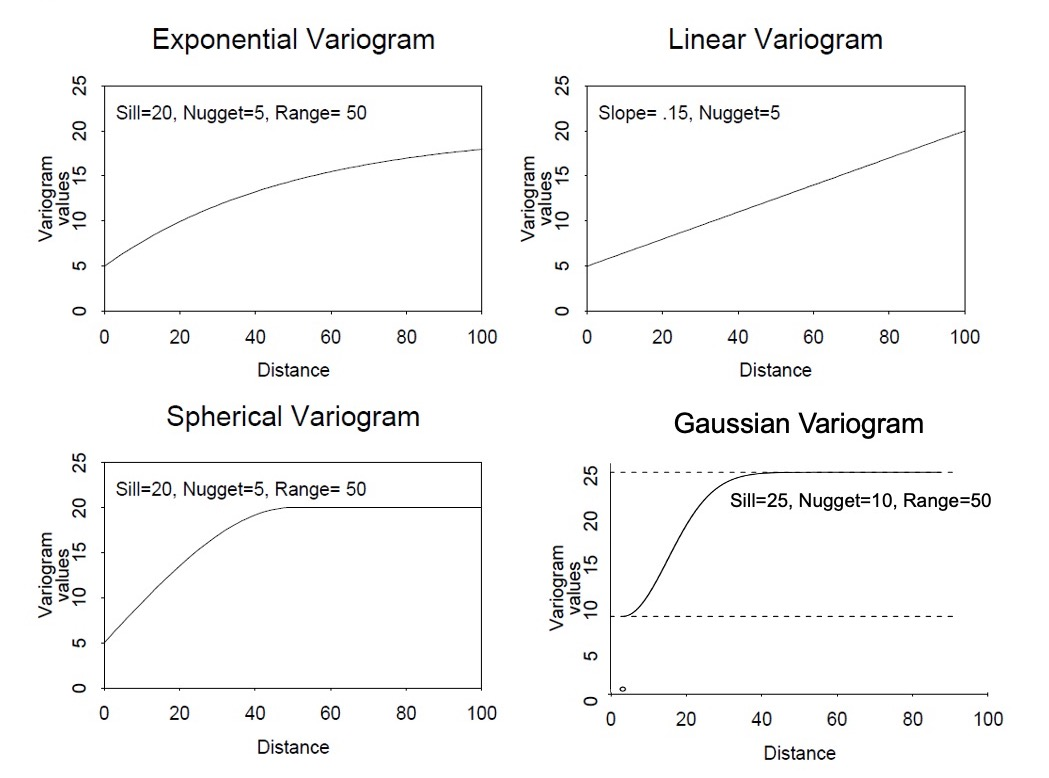
\includegraphics[width=\textwidth]{VariogramModels}
          \end{center}
\end{frame}


\begin{frame}
\frametitle{Examples of variogram models}
    \begin{center}
     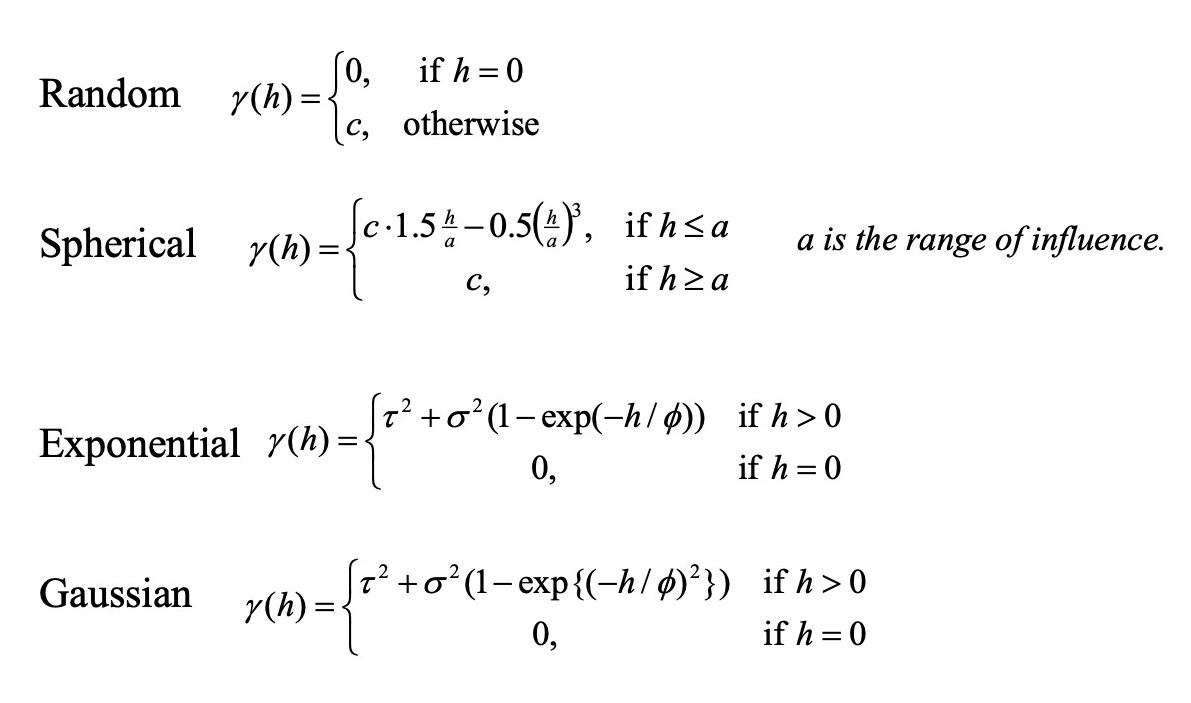
\includegraphics[width=\textwidth]{VariogramFormulae}
          \end{center}
\end{frame}

\begin{frame}
\frametitle{Notation}
 \begin{itemize}
\item The key features of our variogram are represented by the following model parameters
\begin{itemize}
\item $\tau^2 > 0$ is the \textbf{nugget}.
\item $\sigma^2 > 0$ is the \textbf{partial sill}.
\item $\phi > 0$ is the \textbf{range parameter}.
\end{itemize}
\vspace{3mm}
\item Note that $\phi$ is not the range itself, but rather a parameter which controls how quickly the covariance decays towards zero (or the variogram increases to the sill).
\vspace{3mm}
\item A smaller value of $\phi$ means the covariance function decays to zero quickly, a larger value means it decays to zero more slowly.
\end{itemize}
\end{frame}


\begin{frame}
\frametitle{Example - Meuse river}
\begin{itemize}
\vspace{2mm}
\item We can now fit a variogram model to the empirical variogram obtained from the Meuse river example.
\vspace{3mm}
\item The black solid line below shows an exponential variogram model (fitted using the \texttt{geoR} package).
\end{itemize}
    \begin{center}
     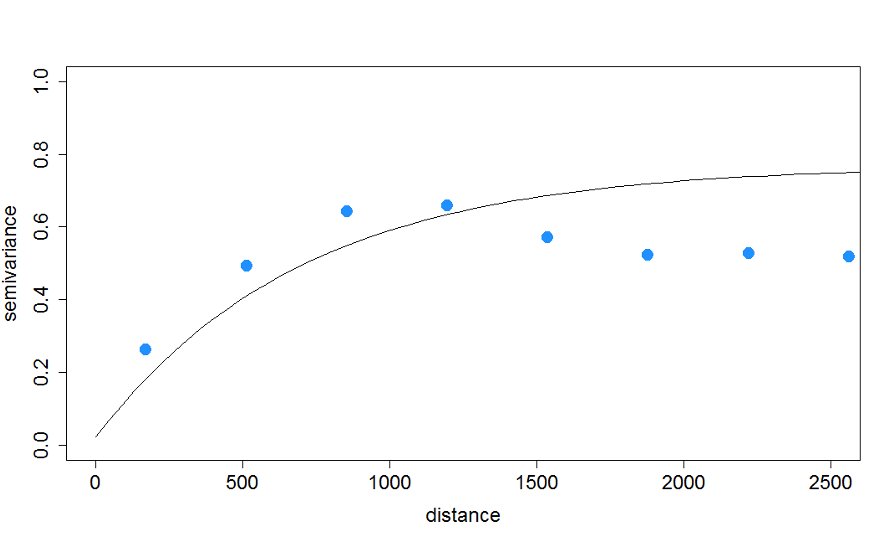
\includegraphics[width=0.85\textwidth]{MeuseModel}
          \end{center}
\end{frame}


\begin{frame}
\frametitle{Prediction}
 \begin{itemize}
\item Once we have estimated a variogram to account for our spatial autocorrelation, we can start to think about making predictions.
\vspace{3mm}
\item Spatial prediction is the process of predicting the value of our variable of interest at an unobserved location $\bd{s}_0$.
\vspace{3mm}
\item As with any statistical prediction, we use what we know about our observed data, including their values, how far our unobserved location is from them, and our variogram.
\vspace{3mm}
\item There are many methods for spatial predictio, including regression modelling, distance weighted interpolation and an approach known as \textbf{kriging}.
\end{itemize}
\end{frame}


\begin{frame}
\frametitle{Kriging}
 \begin{itemize}
\item Kriging is an approach named after its inventor D. G. Krige, who worked in the mining industry in South African in the 1950s.
\vspace{3mm}
\item He used this approach to understand the spatial pattern of mineral resources.
\vspace{3mm}
\item It is a relatively simple and theoretically appealing approach, and is therefore incredibly popular for geostatistical prediction.
\vspace{3mm}
\item Kriging interpolates between previously observed locations in order to predict at new locations. 
\end{itemize}
\end{frame}

\begin{frame}
\frametitle{Ordinary Kriging}
 \begin{itemize}
\item Ordinary kriging is a form of kriging which assumes that the overall mean and variance of the region is constant.
\vspace{3mm}
\item Predictions at unsampled locations are made using a weighted average of the observations. $$z^*(\bd{s}_0) = \sum_{i=1}^m \lambda_i z(\bd{s}_i)$$
\item The weights $\lambda_i$ can be estimated in a number of different ways, and are commonly based on the variogram.
\vspace{3mm}
\item The weights are therefore usually proportional to the distance between the observed and new locations.
\end{itemize}
\end{frame}


\begin{frame}
\frametitle{More on Kriging}
 \begin{itemize}
\item There are other types of kriging such as \emph{universal kriging} and \emph{block kriging} which are more appropriate for different structures of spatial data.
\vspace{3mm}
\item Whichever method is used, we can obtain a set of predictions over a grid to allow us to plot a map of the predicted spatial surface for our variable of interest.
\vspace{3mm}
\item Our predictions will be of better quality in areas where there are lots of observed values, and poorer quality when we have less nearby data available.
\vspace{3mm}
\item Therefore we can also generate a map of the uncertainty across the region. 
\end{itemize}
\end{frame}


\begin{frame}
\frametitle{Predicted Surface}
 \begin{itemize}
 \vspace{1mm}
\item The surface map on the right is generated by using kriging to make predictions over a fine grid.
\vspace{3mm}
\item Notice the `edge effects' - a gradual smoothing towards the mean as you move away from any actual data in the top left and bottom right.
\end{itemize}
\vspace{-2mm}
\begin{columns}
\begin{column}{0.5\textwidth}
    \begin{center}
     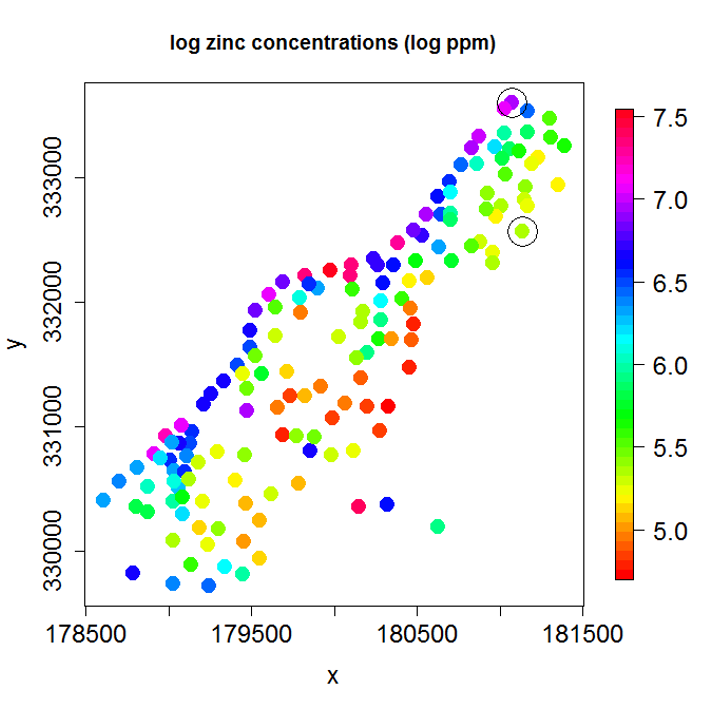
\includegraphics[width=\textwidth]{MeusePoints}
          \end{center}
\end{column}
\begin{column}{0.5\textwidth}
    \begin{center}
     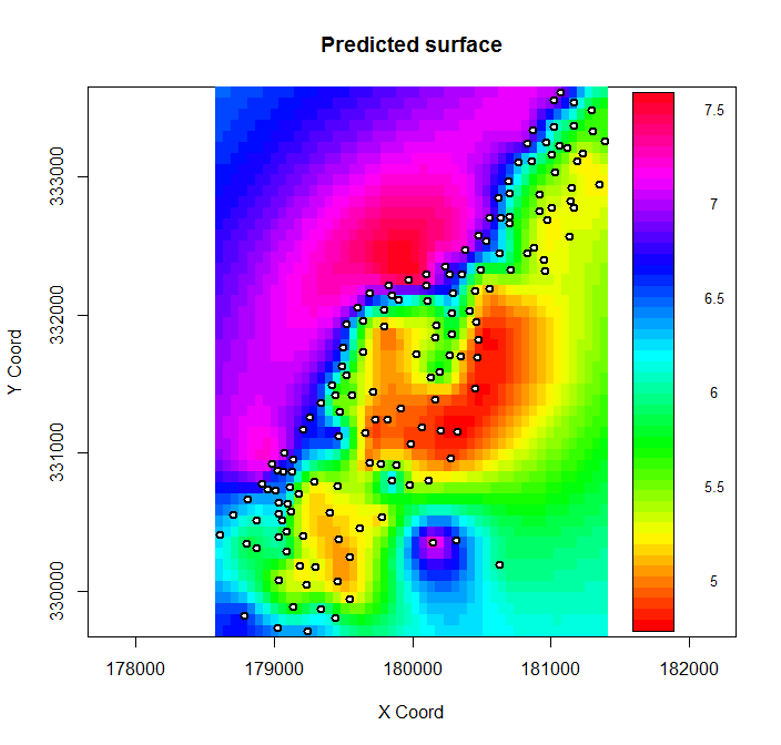
\includegraphics[width=\textwidth]{MeuseSurface}
          \end{center}
\end{column}
\end{columns}
\end{frame}


\begin{frame}
\frametitle{Uncertainty}
 \begin{itemize}
 \vspace{1mm}
\item The map on the left shows the uncertainties associated with our estimated surface.
\vspace{3mm}
\item There is lower uncertainty in the areas with lots of observed data, and higher uncertainty as we move away from the observed data.
\end{itemize}
\vspace{-2mm}
\begin{columns}
\begin{column}{0.5\textwidth}
    \begin{center}
     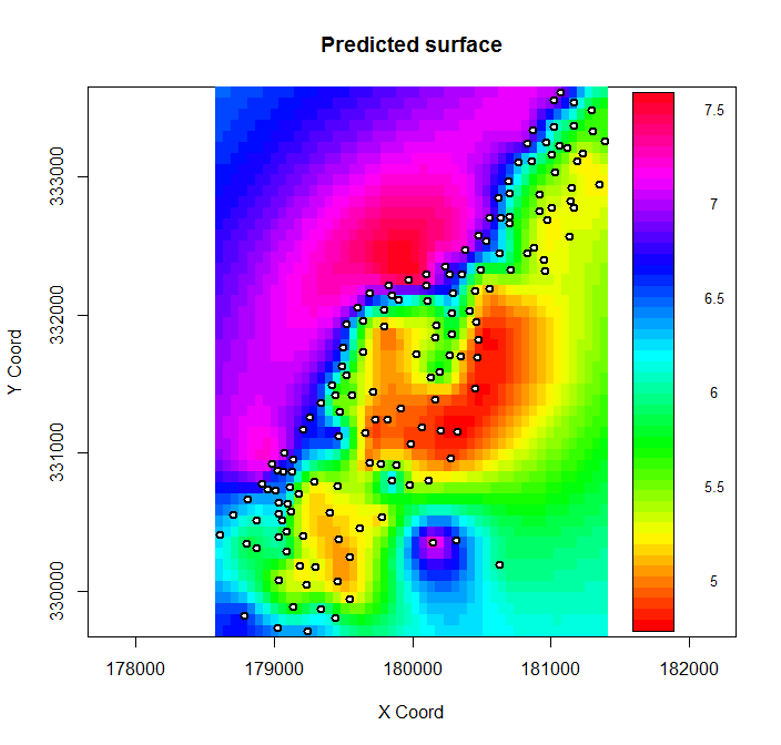
\includegraphics[width=\textwidth]{MeuseSurface}
          \end{center}
\end{column}
\begin{column}{0.5\textwidth}
    \begin{center}
     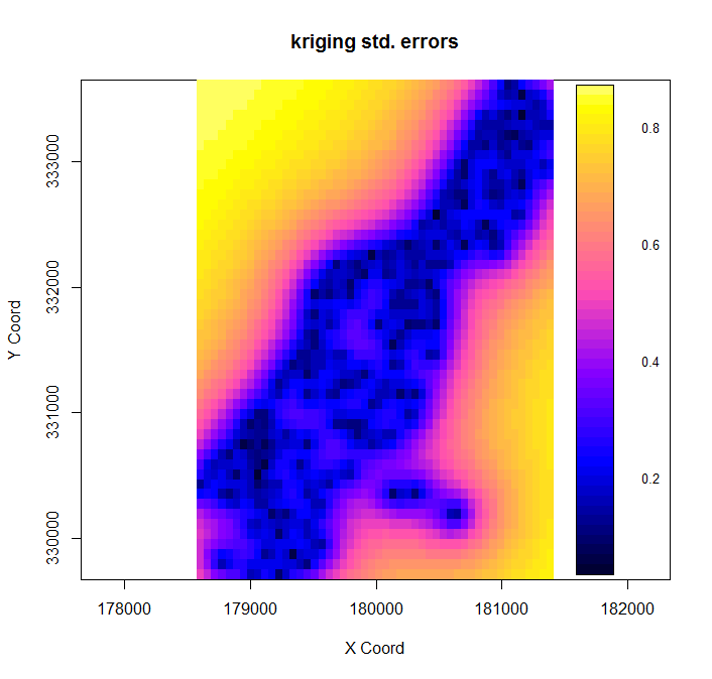
\includegraphics[width=\textwidth]{MeuseErrors}
          \end{center}
\end{column}
\end{columns}
\end{frame}

\begin{frame}
\frametitle{Geostatistical modelling - summary}
 \begin{itemize}
\item When working with geostatistical data, we first have to understand what sort of spatial trend, if any, is present in our data. 
\vspace{3mm}
\item Next, we plot the empirical (semi-)variogram and choose a suitable model structure.
\vspace{3mm}
\item We then identify the parameters (sill, nugget, range) of this chosen model structure.
\vspace{3mm}
\item Finally, we use this model to obtain weights which can be used for interpolation via, for example, kriging, and use this to estimate the surface on a map.
\end{itemize}
\end{frame}

\begin{frame}
\frametitle{\textcolor{orange}{Treat People With Kindness}}
\center{

\includegraphics[scale=0.22]{Menti-W6-2}\\
}
\vspace{-3mm}
\url{https://www.menti.com/alws53ba6bzm}
\end{frame}
  

\end{document}



